% This is a template for Ph.D. dissertations in the UCI format.
% 
% All fonts, including those for sub- and superscripts, must be 10
% points or larger.  Recommended sizes are 14-point for chapter
% headings, 12-point for the main body of text and figure/table
% titles, and 10-point for footnotes, sub- and super-scripts, and text
% in figures and tables.
%
% Notes: Add short title to figures, sections, via square brackets,
% e.g. \section[short]{long}.
%
\documentclass[12pt,fleqn]{ucithesis}

% A few common packages
\usepackage{amsmath}
\usepackage{amsthm}
\usepackage{array}
\usepackage{graphicx}
\usepackage{natbib}
\usepackage{relsize}

% Some other useful packages
\usepackage{caption}
\usepackage{subcaption}  % \begin{subfigure}...\end{subfigure} within figure
\usepackage{multirow}
\usepackage{tabularx}

% plainpages=false fixes the "duplicate ignored" error with page counters
% Set pdfborder to 0 0 0 to disable colored borders around PDF hyperlinks
\usepackage[plainpages=false,pdfborder={0 0 0}]{hyperref}

% Uncomment the following two lines to use the algorithm package,
% which provides an algorithm environment similar to figure and table
% ("\begin{algorithm}...\end{algorithm}"). A list of algorithms will
% automatically be added in the preliminary pages. Note that you
% probably want a package for the actual code to go with this (e.g.,
% algorithmic).
%\usepackage{algorithm}
%\renewcommand{\listalgorithmname}{\protect\centering\protect\Large LIST OF ALGORITHMS}

% Uncomment the following line to enable Unicode support. This will allow you
% to enter non-ASCII characters (such as accented characters) directly without
% having to use LaTeX's awkward escape syntax (e.g., \'{e})
% NOTE: You may have to install the ucs.sty package for this to work. See:
% http://www.unruh.de/DniQ/latex/unicode/
%\usepackage[utf8x]{inputenc}


% Modify or extend these at will.
\newtheorem{theorem}{{\sc Theorem}}[chapter]
\newtheorem{definition}{{\sc Definition}}[chapter]
\newtheorem{example}{{\sc Example}}[chapter]

% Uncomment the following to have numbered subsubsections (by default
% numbering goes only to subsections).
%\setcounter{secnumdepth}{4}


% Set this to only select a subset of the includes directives below.
% Very handy to speed up compilation if you're working on a certain
% part of your thesis. It conserves page numbers, references, etc.
% even for non-included files.
%\includeonly{chapter1}

\begin{document}

% Preliminary pages are always loaded (TOC, CV, etc.)
% \thesistitle{
%   Pruning Large Search Spaces using Context Networks
% }

\thesistitle {
  Discovering Real World Context to Tag Personal Photos
}

\degreename{Doctor of Philosophy}

% Use the wording given in the official list of degrees awarded by UCI:
% http://www.rgs.uci.edu/grad/academic/degrees_offered.htm
\degreefield{Computer Science}

% Your name as it appears on official UCI records.
\authorname{Arjun Satish}

% Use the full name of each committee member.
\committeechair{Professor Ramesh Jain}
\othercommitteemembers
{
  Dr. Amarnath Gupta\\
  Professor Nalini Venkatasubramanian\\
  Professor Deva Ramanan\\
  Professor Bill Tomlinson
}

\degreeyear{2013}

\copyrightdeclaration
{
  {\copyright} {\Degreeyear} \Authorname
}

% If you have previously published parts of your manuscript, you must list the
% copyright holders; see Section 3.2 of the UCI Thesis and Dissertation Manual.
% Otherwise, this section may be omitted.
% \prepublishedcopyrightdeclaration
% {
% 	Chapter 4 {\copyright} 2003 Springer-Verlag \\
% 	Portion of Chapter 5 {\copyright} 1999 John Wiley \& Sons, Inc. \\
% 	All other materials {\copyright} {\Degreeyear} \Authorname
% }

% The dedication page is optional.
\dedications
{
  \textit{And it's whispered that soon, if we all call the tune,} \\
  \textit{Then the piper will lead us to reason} \\
  \textit{And a new day will dawn for those who stand long} \\
  \textit{And the forest will echo with laughter} \\ 
  \textit{} \\
  \setlength{\parindent}{6.3cm} \texttt{Jimmy Page \& Robert Plant, } \\
  \setlength{\parindent}{7cm} \texttt{from Stairway to Heaven, 1970} \\
}

\acknowledgments
{

I would like to thank my advisors, Ramesh Jain and Amarnath Gupta for teaching me the values and fundamental principles of the scientific method. Without their continuing support, a project like CueNet would have barely made this far. The many technical and personal discussions I had with them during the last few years are going to be greatly missed. I owe a lot to Ramesh for accepting me as a graduate student, and introducing me to his beloved projects and ideas and letting me play with them as I seemed fit.

Special thanks to my committee members, Deva Ramanan, Nalini Venakatasubramian and Bill Tomlinson to take the time out to provide feedback on my work and suggesting very interesting experiments which helped me gain some major insights into it. My fellow graduate students at ISG were always a source of inspiration and encouragement to work on challenging cross-domain problems. 

My friends at the Experiential Systems Laboratory: Setareh, Hamed, Laleh and Siripen deserve a huge reward for putting up with me these past few years. They have always been extremely supportive and took the time to provide enormous amounts of feedback and ideas to improve all the projects I have worked on. Many thanks to them for helping shape the ideas presented in the following pages.

A special thanks to Alex Thornton, Chen Li and Mike Carey to help me understand the teacher's side of the table at universities. Working with them has helped me understand how I can change the world in small steps by guiding students the right way. Big thanks to the students whom I worked with during the last five years here. 

I owe my best friends Shekhar and Karthik for patiently bearing my tantrums for the last decade. Without Shekhar’s persistent pushes, I would have never applied to graduate school. Big thanks to them for introducing me to the world of music, which colors many of the gray days.

Hearty thanks to Amrish, Ronen and Liat to introducing me to various events during my first days at the USA. They helped me explore various aspects of life in UCI, which I would have never been exposed to otherwise.

A big thanks to my dear friends Alex, Nick, Stephanie, Vinnie, Joel, Ashley, Sameer, Alegria and Reuben for all the barbecues, wine nights, dessert parties, concerts and all the other kinds of activities which made the last few years so memorable. A small apology to Alex and Nick for stopping them halfway each time we decided to run a few miles together.

Sincerest thanks to my family, and friends, Shweta, Sidharth and Natasha for helping me through the ups and downs of life. This dissertation would have been impossible without your help. 

}


% Some custom commands for your list of publications and software.
\newcommand{\mypubentry}[3]{
  \begin{tabular*}{1\textwidth}{@{\extracolsep{\fill}}p{4.5in}r}
    \textbf{#1} & \textbf{#2} \\ 
    \multicolumn{2}{@{\extracolsep{\fill}}p{.95\textwidth}}{#3}\vspace{6pt} \\
  \end{tabular*}
}
\newcommand{\mysoftentry}[3]{
  \begin{tabular*}{1\textwidth}{@{\extracolsep{\fill}}lr}
    \textbf{#1} & \url{#2} \\
    \multicolumn{2}{@{\extracolsep{\fill}}p{.95\textwidth}}
    {\emph{#3}}\vspace{-6pt} \\
  \end{tabular*}
}

% Include, at minimum, a listing of your degrees and educational
% achievements with dates and the school where the degrees were
% earned. This should include the degree currently being
% attained. Other than that it's mostly up to you what to include here
% and how to format it, below is just an example.
\curriculumvitae
{

\textbf{EDUCATION}
  
  \begin{tabular*}{1\textwidth}{@{\extracolsep{\fill}}lr}
    \textbf{Doctor of Philosophy in Computer Science} & \textbf{2013} \\
    \vspace{6pt}
    University of California, Irvine & \emph{Irvine, CA} \\
    \textbf{MS in Computer Science} & \textbf{2011} \\
    \vspace{6pt}
    University of California, Irvine & \emph{Irvine, CA} \\
    \textbf{BE in Electronics and Communications} & \textbf{2002-2006} \\
    \vspace{6pt}
    Sir MV Institute of Technology & \emph{Bangalore, Karnataka, India} \\
  \end{tabular*}

\vspace{12pt}
\textbf{RESEARCH EXPERIENCE}

  \begin{tabular*}{1\textwidth}{@{\extracolsep{\fill}}lr}
    \textbf{Graduate Research Assistant} & \textbf{2007--2013} \\
    \vspace{6pt}
    University of California, Irvine & \emph{Irvine, California} \\
    \textbf{Research Intern} & \textbf{2010} \\
    \vspace{6pt}
    Microsoft Research & \emph{Mountain View, California} \\
  \end{tabular*}

\vspace{12pt}
\textbf{TEACHING EXPERIENCE}

  \begin{tabular*}{1\textwidth}{@{\extracolsep{\fill}}lr}
    \textbf{Teaching Assistant} & \textbf{2007--2013} \\
    \vspace{6pt}
    University of California, Irvine & \emph{Irvine, California} \\
  \end{tabular*}

\vspace{12pt}
\textbf{SELECTED HONORS AND AWARDS}

  \begin{tabular*}{1\textwidth}{@{\extracolsep{\fill}}lr}
    \textbf{Google, Ph.D. Fellowship} & \textbf{2012} \\
    \vspace{6pt}
    Google, Inc.\\

    \textbf{Hitec Octane Entrepreneurship Competition} & \textbf{2008} \\
    \vspace{6pt}
    Second Prize & \emph{Irvine, California} \\
  \end{tabular*}

\pagebreak

\textbf{REFEREED CONFERENCE PUBLICATIONS}

  \mypubentry{CueNet: a Context Discovery Framework to Tag Personal Photos}{Mar 2013}{ICMR 2013}  
  \mypubentry{Visualizing Progressive Discovery}{Mar 2013}{ICMR 2013}  
  \mypubentry{Tolkien: An Event Based Storytelling System}{Aug 2009}{VLDB 2009}
  \mypubentry{A New Approach for Adding Browser Functionality}{Jun 2008}{Hypertext 2008}

\vspace{12pt}
\textbf{TECHNICAL REPORTS}

  \mypubentry{Context Networks for Annotating Personal Media}{May 2013}{ESL.UCI.EDU-TR 2013-May/01}
  \mypubentry{Tagging Personal Photos Using Contextual Information}{Aug 2012}{Whitepaper}
  \mypubentry{Lives: A System for Creating Families of Multimedia Stories}{Aug 2010}{MSR-TR-2011-65}
  \mypubentry{Tolkien: Weaving Stories from Personal Media}{Jun 2010}{ESL.UCI.EDU-TR 2010/04/11}

\vspace{12pt}
\textbf{SOFTWARE}

  \mysoftentry{CueNet}{https://github.com/wicknicks/cuenet/}
  {Polyglot implementation of the CueNet ecosystem to tag faces in photos.}

}

% The abstract should not be over 350 words, although that's
% somewhat of a soft constraint.
\thesisabstract
{
Automatic annotation algorithms assign one or more labels from a candidate search space to a given input object. The collection of these labels is either constructed manually, or derived from a set of sources. It is known that the accuracy of annotation algorithms is typically a decreasing function of the number of labels in the search space. In annotating real-world multimedia objects, this search space quickly explodes if not carefully curated. In this work, we present a technique to prune search spaces yet retain a very large number of correct tags for a multimedia object. Specifically, we shall address pruning of search spaces for the problem of tagging faces in the photo media.

Photos capture the momentary state of real-world entities. Any knowledge of the state of entities in the real world at the time of photos capture provides useful context to eliminate candidates in the search space. For example, people in Japan cannot appear in photos taken at Paris, and photos taken at an academic conference will largely contain people who work in the same field. 

In the real world, relations between entities change rapidly. It is not possible to use a static model of entity relationships to reason over faces in photo instances taken across a wide range of time. Thus, it is imperative that any system first \textit{discover} the set of relationships which are true at the time of photo capture before pruning the search space.

In this dissertation, we adopt a \textbf{relation-centric view} of real-world contextual information to design and implement a framework, \textbf{CueNet} to discover real-world context. The primary contribution of this dissertation is a \textbf{progressive discovery algorithm} to identify relationships between real-world events and objects. CueNet uses these relationships to reason which objects could appear in a given photos, and uses image features to confirm its hypotheses. People often co-occur across photos. We present a method to \textbf{propagate} objects from neighboring photos to a new untagged photo. We shall extend the concepts behind the PageRank algorithm, used to rank web pages, to order real-world objects, and design score propagation techniques based on event semantics. We present \textbf{experiments} on both real-world photos and simulated events. We implement a system using CueNet to tag thousands of personal photos captured by multiple users, to study the efficacy of using context discovery in pruning search spaces. We also present simulation experiments to measure the time and space complexity of large scale discovery operations. We present the convergence characteristics and results on our real-world datasets to show the utility of the propagation algorithm. 

Finally, we conclude the dissertation by presenting challenging problems for future research and ideas for new applications which can be designed using the foundations of context discovery techniques.
}


%%% Local Variables: ***
%%% mode: latex ***
%%% TeX-master: "thesis.tex" ***
%%% End: ***

\preliminarypages

% Include the different components of your thesis, in separate files.
% Using \include allows you to set \includeonly above.
\chapter{Introduction}

This dissertation introduces a new approach to discovering context for photo annotation problems. The primary complexity of photo annotation problems lie in their large search spacesand the diversity of feature-based representations of images. Contextual information is used to prune this large search spaces with reduced dependency on image features. Once the search space has been reduced, the image features are used to select from the \textit{remaining} tags. For example, people with weak social ties do not co-occur often in photos, and by identifying one we can eliminate the other. In this case, we would say that social context is used to prune candidates in a face annotation problem.

Recently, there have been two changes in the scientific community which motivates us to take a fresh look at context. First, with mobile phones becoming the primary mode of photo taking, the nature of context has evolved from providing cues about tags, to the description of the world around a photo taking moment when a person was taking the photo. With the ever increasing amount of personal, social and public information, it is becoming harder to specify which subset of these would constitute the most interesting context for a given picture. Thus, it is not clear what data to consider context, and how do we combine them to form models of the real world which will allow photo annotation algorithms to reason what tags to assign various regions in a given photo.

More specifically, we address the problem of constructing computational representations of real world events from various heterogeneous data sources, to reason which parts of the search space can be pruned without hurting the overall performance of the annotation algorithm. We refer to such a representation as the \textbf{Context Network} of the photo. The network describes real-world events occurring in the environment, the entities participating in them, and their semantic inter-relationships.

\begin{figure}[t]
\centering
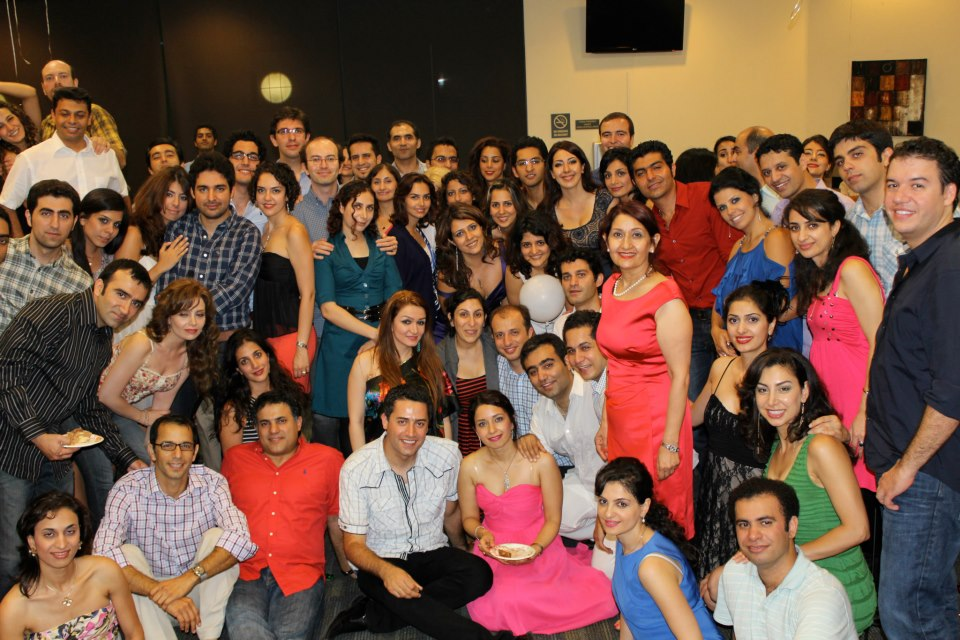
\includegraphics[width=0.8\textwidth]{media/chapter1/setarehetal}
\caption{Face tagging problems could be challenged by very large search spaces.}
\label{fig:people}
\end{figure}

\section{Importance of Context Discovery}

Computer science is moving towards solving real world problems. Social network analysis, medical diagnosis prediction, philanthropic engineering, monitoring public interests through real time communication networks, and situation-based advertising are some of the emerging applications in our area. The common requirement for all of them is to construct models of the real world events occurring in the world, who is participating in them and their attributes and relationships. A technology to construct such a model from various data sources currently available today can play a key role in the effective functioning of such systems.

For the purposes of this dissertation, we propose context discovery techniques in the light of photo annotation problems alone, but the technology and ideas are not tightly coupled with any singly media, and can be easily migrated to assist in solving any problem which requires models of real world events.

\section{Novelty}

Context has been used to address many multimedia problems \cite{henter2012tag, li2012fusing, naaman2005identity, o2009context,stone2008autotagging}. For example, time and location information or social network information from Facebook to solve the face recognition problem. We refer to such a direct dependency between the search space and a data source as \textbf{static linking}. Although these systems are meritorious in their own right, they suffer from the following drawbacks: they are tightly coupled with a few data sources, the unavailability of which would reduce the efficiency of the system, do not employ multiple sources, and therefore the \textbf{relations} between them. 

\begin{figure}[t]
\centering
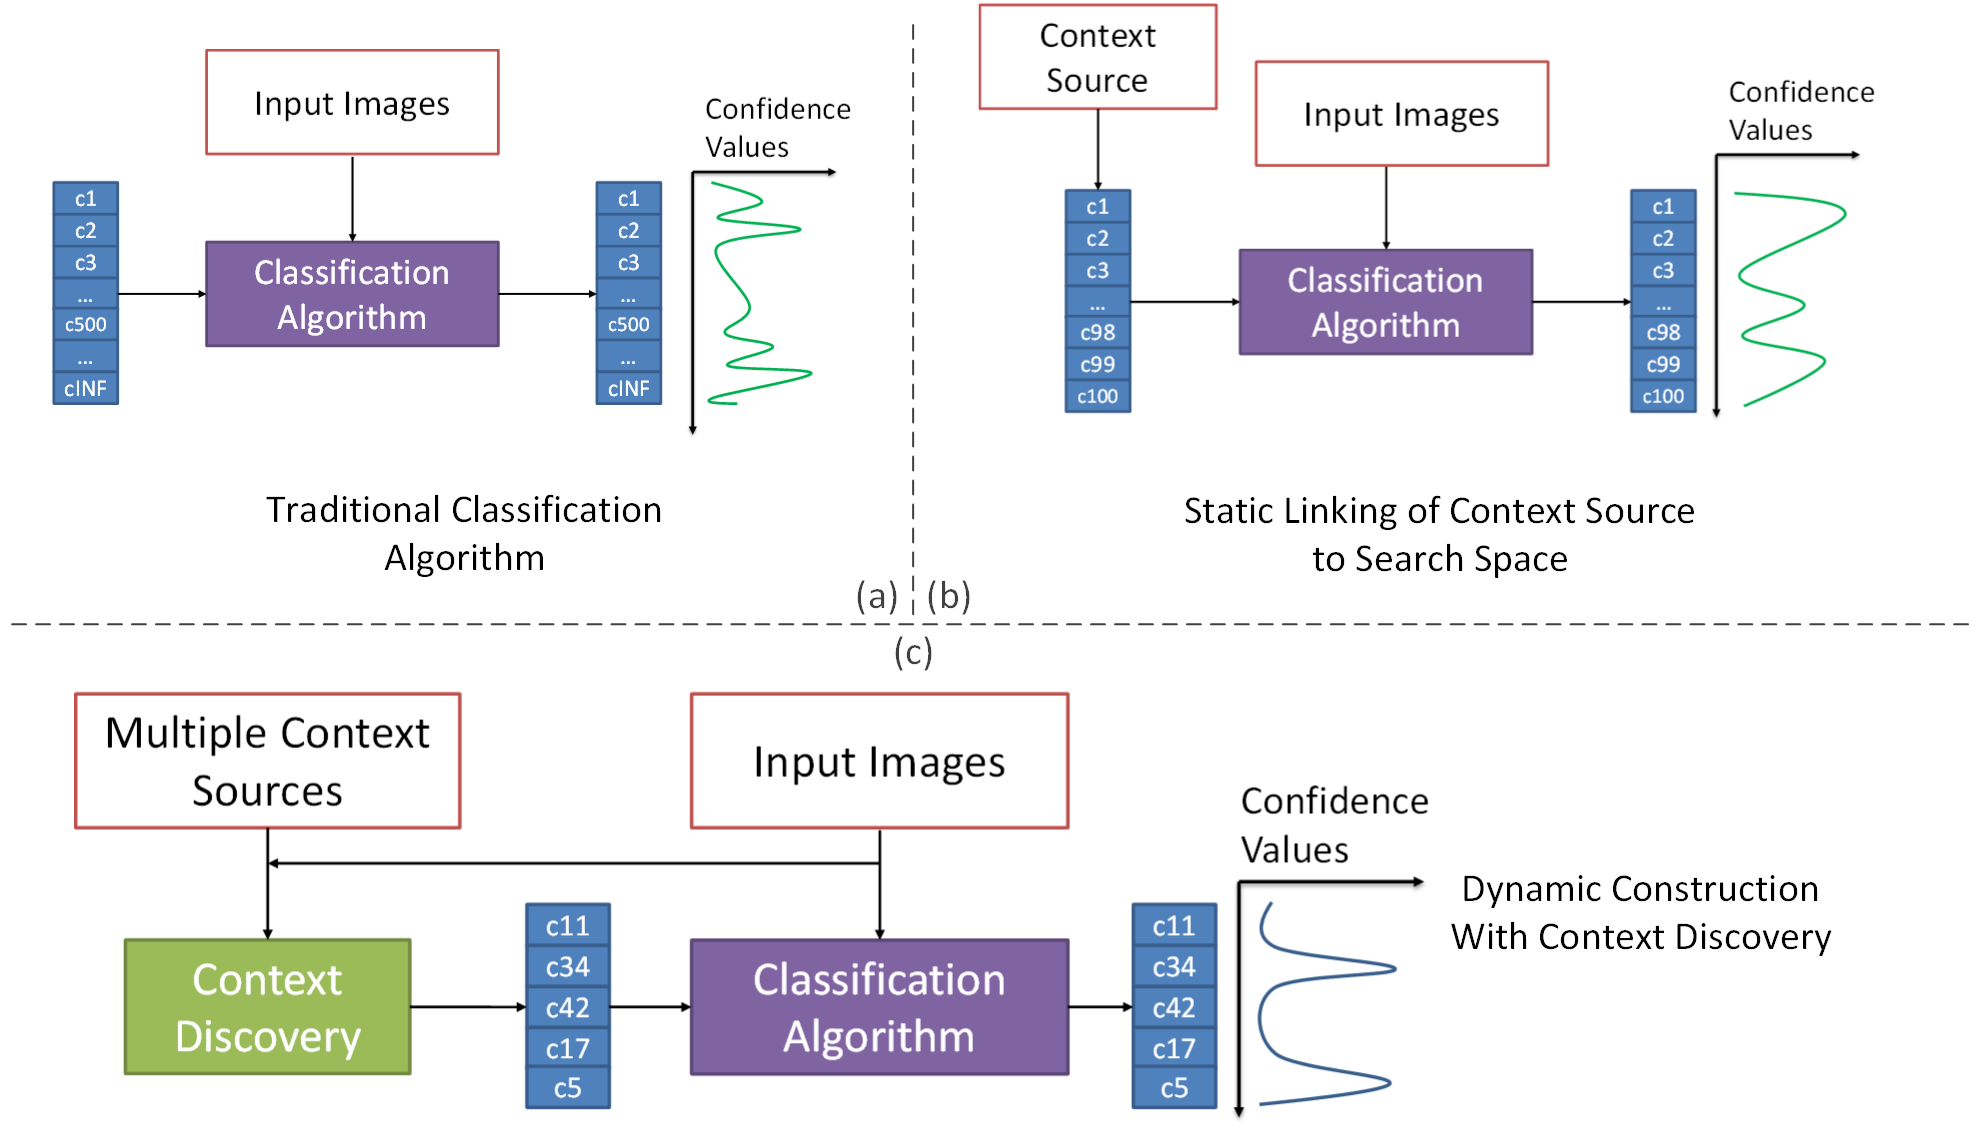
\includegraphics[width=0.85\textwidth]{media/with-without-cuenet-2.png}
\caption{The different approaches in search space construction for a multimedia annotation problem.}
\label{fig:with-without-cuenet}
\end{figure}

Figure \ref{fig:with-without-cuenet} shows the three major ways to prune search spaces in annotation systems. Figure \ref{fig:with-without-cuenet}(a) is one of the earliest system setups where the search spaces were manually constructed, and the focus was mainly on constructing smarter features to correctly classify feature sets \cite{turk1991eigenfaces, belhumeur1997eigenfaces}. Systems like \cite{stone2008autotagging} use a single source like Facebook to populate their search space based on some attributes of the input problem (in this case, the identity of the user). This restricted the search space but it is assumes that all relevant tags will be supplied from the context source, which is usually not correct.

This primary \uline{contribution} of this dissertation is a \textbf{\textit{progressive discovery}} algorithm to ingest information from various real world data sources to construct context networks containing the most relevant information for pruning the search space for the system. Examples of data sources include social media web services to provide information about events and entities like Facebook, Twitter; services which can be queried to find information about places like Yelp; Sensors on personal mobile phones, for example GPS which inform applications of the location of a person is present at any given point in time.

\section{Approach}

\textbf{What is progressive discovery?} Progressive discovery is an incremental process where knowledge of real world events and entities can be added to a given context network. Given a context network and multiple data sources describing events and entities, a progressive discovery algorithm will obtain new information from the sources and relate it to context network. By iteratively executing this algorithm, we can grow a context network until the data sources can provide no further information or the information in the network prunes the search space well enough for the AI problem to be fully solved.

The discussion in the following chapters on context networks and their discovery from various data sources will be presented in conjunction with an application to \textbf{tag faces in personal photos}. The face tagging algorithm, whose search space contains a few million entities attempts to solve a very hard problem. But if a real world model of the world existed, the search space which is relevant to this photo contains just the entities who are present within the field of view of the camera at the time the photo was captured. 

\section{Examples}
Here are two examples of dynamic linking. Figure \ref{fig:example-icmr-hidden} shows a photo of a person about to starting his presentation. Dynamic linking is done in three steps. First, the discovery algorithm proceeds to find the EXIF parameters of the photo, and associates the user with the photo. We call such an event where a photo is associated with its spatio-temporal attributes, a \texttt{photo-capture-event}. It signifies an event where the user is capturing an image with his camera. Second, these attributes are used to discover \textit{what is other events is the owner part of at this time}? Only those data sources are queried which can provide answers to this, and we obtain a response from a conference database saying that the owner was attending the ICMR conference at Dallas, Texas. Third, given this new conference event, the algorithm discovers what were the conference subevents (like keynotes, talks or break sessions) were occurring at this time. Finally, it finds that Mor Naaman and John Smith were speaker and host for the keynote talk going on that time. Given the two candidates, the face tagging algorithm proceeds to identify the correct tag, figure \ref{fig:example-icmr-show}.


\begin{figure}[ht]
\begin{minipage}[b]{0.45\linewidth}
\centering
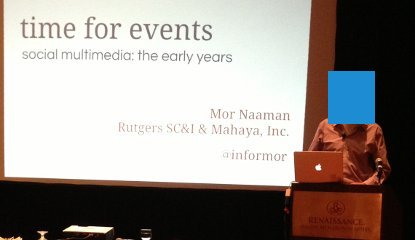
\includegraphics[width=\textwidth]{media/chapter1/icmr-keynote-2-hidden.jpg}
\caption{Who is in this photo?}
\label{fig:example-icmr-hidden}
\end{minipage}
\hspace{0.5cm}
\begin{minipage}[b]{0.45\linewidth}
\centering
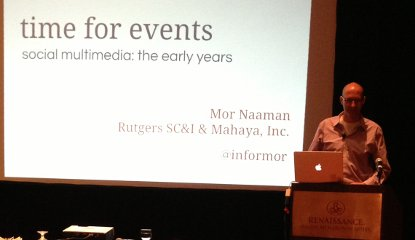
\includegraphics[width=\textwidth]{media/chapter1/icmr-keynote-2-show.jpg}
\caption{Mor Naaman at ICMR.}
\label{fig:example-icmr-show}
\end{minipage}
\end{figure}

Now, lets look at in photo in figure \ref{fig:example-kasturi-hidden}. Context discovery initiates the same way as in the above example, but after searching for events related to the owner in data sources, finds nothing. It proceeds to rank all known contacts according to location, and given that this photo was taken to the owner's workplace ranks colleagues higher than friends. The top 20 (an arbitrary constant) ranked candidates are passed to the face tagging algorithm which finds Ramesh Jain in the photo. But not the person to his right in the photo. But now, the \texttt{photo-capture-event} has an additional participant, Ramesh, whose calendar can be queried to find events in which he was participating. The calendar returns the entry ``Kasturi". The algorithm uses this term to find all Ramesh's contacts to find all people with first or last name ``Kasturi'', and finds his long time friend and colleague ``Rangachar Kasturi''. The face tagging algorithm is invoked with one candidate.

\begin{figure}[ht]
\begin{minipage}[b]{0.45\linewidth}
\centering
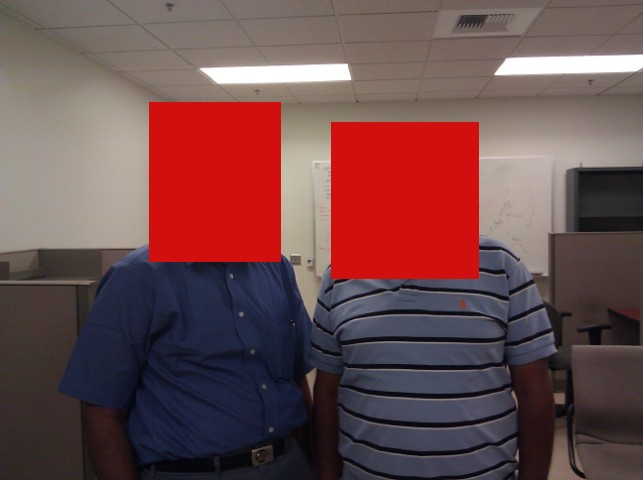
\includegraphics[width=\textwidth]{media/chapter1/kasturi-hidden.jpg}
\caption{Who is in this photo?}
\label{fig:example-kasturi-hidden}
\end{minipage}
\hspace{0.5cm}
\begin{minipage}[b]{0.45\linewidth}
\centering
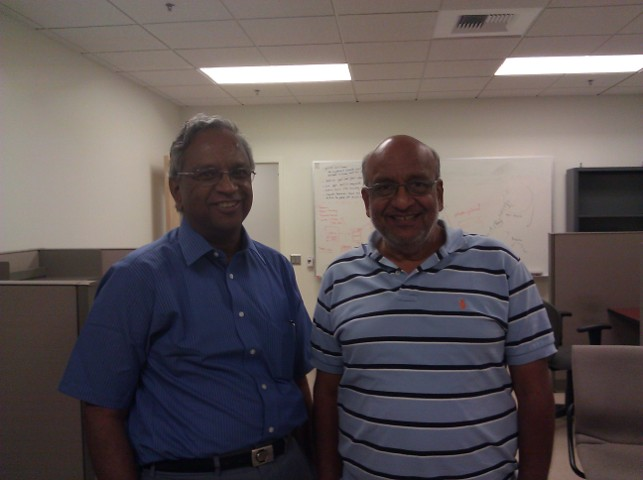
\includegraphics[width=\textwidth]{media/chapter1/kasturi-show.jpg}
\caption{Kasturi and Jain.}
\label{fig:example-kasturi-show}
\end{minipage}
\end{figure}

In this first run, the algorithm linked only to a conference database, whereas in the second case, it used spatial information, personal calendar and contact information. In the later chapters, we will present techniques to represent and link context in a systematic manner.

\section{Overview}
This dissertation is organized into the following chapters. Chapter 2 provides an overview of context, how context has been used to address problems in various scientific disciplines and how we use context in our specific personal photo tagging application. Chapter 3 describes the related work in computer science, and how this work is informed by them. Chapter 4 describes our context discovery framework, how it models various data sources, and how our progressive discovery algorithm constructs models for real world problems. We facilitate this discussion with an example real world application to tag faces of people in personal photos. Chapter 5 analyzes the algorithmic complexity of different parts of the system, and provides experiments to verify the competence and performance of the system. We also present experiments to confirm the efficacy of our approach in the light of the real world application. Finally, chapter 6 attempts to describe the future possibilities of using context discovery in computer science.

% Chapters 6 and 7 describe two extensions to the CueNet framework to solve problems of missing context and that of source selection. 

%% \section{Terminology}
%% Before starting the discussion on Context Networks, it is necessary to include a short note on terminology to avoid any ambiguities. We use the word `Object' to collectively refer to events and entities. An entity includes persons, places in the world, for example `Starbucks, UC Irvine', `The Eiffel Tower, Paris, France', or organizations, for example `Google Inc', `Royal Society of London'. The term `object' has been used in literature to refer to things which have no temporal properties. But, in our discussion, an `object' could imply an event which exhibits temporal properties.

% \begin{figure}[h]
% \centering
% 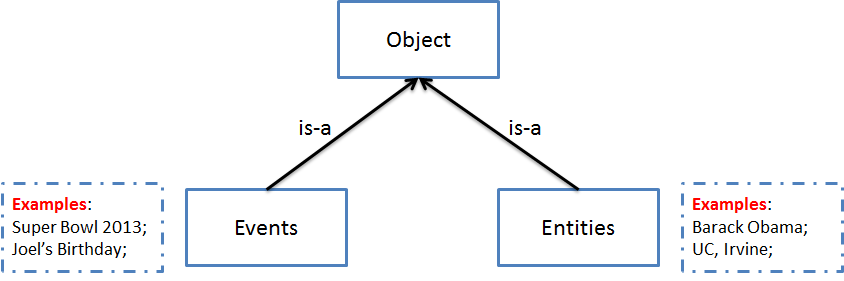
\includegraphics[width=0.75\textwidth]{media/chapter1/terminology.png}
% \caption{Objects, Events and Entities.}
% \label{fig:terminology}
% \end{figure}


% \begin{figure}[ht]
% \begin{minipage}[b]{0.45\linewidth}
% \centering
% 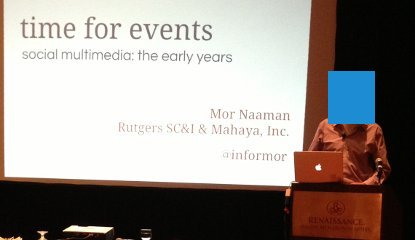
\includegraphics[width=\textwidth]{media/chapter1/icmr-keynote-2-hidden.jpg}
% \caption{Who is in this photo?}
% \label{fig:example-icmr-hidden}
% \end{minipage}
% \hspace{0.5cm}
% \begin{minipage}[b]{0.45\linewidth}
% \centering
% 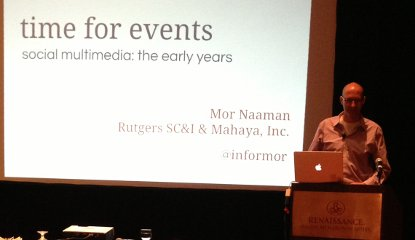
\includegraphics[width=\textwidth]{media/chapter1/icmr-keynote-2-show.jpg}
% \caption{Mor Naaman at ICMR.}
% \label{fig:example-icmr-show}
% \end{minipage}
% \end{figure}

%\chapter{What is Context?}

This chapter describes what we mean by `Context' and `Context-Awareness'. We look at the previous definitions and usages of these terms, and propose why these are lacking for the purposes of this dissertation. As we go through each definition, we will pick out the most relevant parts to form the ground for the context framework introduced in this and developed in later chapters.

\section{Previous Definitons}

The earliest study on context was done by Bill Schilit in 1994, and reported in their paper [CITE]. The focus in this study was how to build software in dynamic environments. The dynamics of the environments were largely due to people requiring computational services, the modality of request (through a mobile device or through a workstation), and the environment of the device (are there cameras and projectors nearby if the task requires video conferencing?). This software-centric view of context highlights the importance of two things. One, context is always described with respect to an object. In this case it is the software which runs on processors distributed in a real world environment. Second, context is used to determine how this object interacts with events and entities near it? For example, Schilit uses the example that a workstation should automatically load his favorite text editor when he approaches it; and an rooster music sample must be played whenever fresh coffee is prepared. Both very different and precise interactions even though they might share common background (environment or participating entities). We would not expect a text editor to be shown when coffee is prepared, and the rooster music to be played when an employee walks to a workstation.

In his seminal paper, Anind Dey [CITE] describes context \textit{as any information that can be used to characterize the situation of an entity. An entity is a person, place or object that is considered relevant to the interaction between a user and an application, including the user and applications themselves.} He proceeds to explain this definition with the example of an ``indoor mobile tour", arguing that there are there are two additional pieces of information which can be used: \textit{weather} and \textit{presence of other people}. if the user is present with his friends, they might visist sites that are of interest to everybody. There the presence of other people is important context. Because the tour is indoor, weather does not affect the application. It is true that the weather has no direct affect on the application but what about the following scenarios:

\begin{itemize}
\item Could we use the weather information to serve different drinks in the cafeteria? On a cold day, placing the hot chocolate kiosk next to the entrance and the ice cream kiosk closer on a warmer day might boost some sales? And add to the overall experience of the tourists?
\item If the tour is similar to Alcatraz, where a ferry ride takes people to the island, and back from it, a storm brewing in the ocean could lead to disrputed ferry services. Should the application warn its users who are liesurely touring at this time? Or should they continue the tour at the same pace, miss the last ferry and spend the night at Alcatraz? After all, accommodation is not a problem.
\end{itemize}

They then proceed to define Context-Aware computing as follows: \textit{A system is context-aware if it uses context to provide relevant information and/or services to the user, where relevancy depends on the user's tasks}. But, we need to ask ourselves why a system which uses this ``additional information" should be considered a context-aware system. There are numerous system which simply would consider these ``additional information" as regular inputs. What is the different between a system which takes in these inputs as processes them as regular data, and one which processes them as context?

Karen Henricksen [CITE] makes the following interesting observation about context: Context information exhibits a range of temporal characteristics. Some context information can be static, for example the attributes of people using a system (for example, the sex of a person). But a large amount of information is dynamic. For example, relations change between people, location and events progress between moments. There is no straightforward way to obtain this dynamic information other than through sensors. But, such a approach tightly couples the application logic to the types of sensors used, and requires the system to convert the input data to usable representations. For example, the application might explicit modules to convert GPS coordinates to readable addresses. The problem with such an approach is that there are many ad-hoc modules built to tackle the sensors, and therefore causing the context-awareness to be tied to a specific application.

More recently, Vaninha Vieira [CITE] uses a knowledge centric view of context to design their context sensitive system, Cemantika. Vaninha defines a contextual element as any piece of data or information which can be used to characterize an entity in an application domain, whereas the context of an interaction between an agent and an application is the set of instantiated contextual elements that are necessary to support the task at hand. Context awareness, for them, is to explicitly change the task which the system is carrying out. For this they explictly model the \textit{context sources} which includes heterogenous and  external sources like sensors, user dialog interfaces and databases. This allows the various processes to operate independently of the type of sources. It should be noted that the use of ontologies is describing knowledge and context sources is becoming increasingly popular. A more listing of relevant work is provided in chapter 3. \textbf{This paves the way for us to bring in the notion of types of information}.

Let us extend the tour guide example to demonstrate the different properties of context. In this extension, we assume that this is the tour guide software to manage a visitor's experience at the Alcatraz Island, San Francisco. The visitor is allowed to walk through the exhibits as s/he pleases, with the tour guide headset providing explanations on the current exhibit, by sensing the current location. The explanations provided are such that they take into consideration what the visitor has already seen at the prison. For example, if the current location requires knowledge of an event which happened at a different section of the prison, then it must not be told. The application must also ensure that all visitors make it to a ferry ride before the last one departs for the day. If there is any problem in that respect, it must present the appropriate data which informs the visitor on the reason for the problem. Since this application knows where every visitor is at a given time, it must ensure that some sections of the Island do not get more crowded that the others. It should either slow down or move the visitors faster if the number of people in a section are increased beyond a particular threshold.

Let's assume that the Island is divided into sections, each of which contains a person counter sensor. The counter sensor can be queried to determine how many people are present in the section. Each visitor carries a handheld device which is capable of sensing its location, and proximity to an exhibit. The ferry maintains a schedule, which is read by the system to make decisions. If there is a problem with the ferry, a maintenance schedule which can be queried to check for any damages to the ferry. We also assume we have access to a local weather channel to check for sudden changes in the weather which might affect the ferry.

When a visitors enters the museum, all sensors are contributing towards the context of the visitor. The person counters are being queried to decide which section the user should move to next, the previous locations are used to form coherent explanations at each new stop. The ferry schedule is checked to make sure there are no disruptions along the way. But what happens when the visitor has finished seeing all the exhibits? We can now ignore all the previous locations, and traffic situation at the different sections. Even though these sensors are in the proximity of the visitor, they are no longer needed. And therefore, contribute no useful context. We can also say \textbf{that the relationships between the visitor, and his environment has changed through time}. Thus, it holds to say that the exact configuration of relationships, at that instant of time, is pivotal in deciding what real world information contributes to context, and what is unecessary.

Relationships can be of different types. They can be simple labels like \texttt{friend-of} signifying a social relationship. Or they can more actionable like \texttt{located-at}, which relates a person to a particular location, and therefore causes a particular audio stream to play through the handheld device. This relation is not just a label, it imposes constraints on the properties of objects which it relates. Here, the spatial attributes of the the person and the exhibit must match if they are being related through a \texttt{located-at} attribute. In this dissertation, we will see that such relations, which impose such property constraints are critical in algorithmically determining which information is relevant context.

We define context of a given object at a particular time as \textbf{``the real world information which can be related to the object directly or indirectly through a known set of relationships''}. Context-awareness of a system is its \textbf{``ability to explore different types of information to identify context relevant to the objects in its ecosystem, and using this additional knowledge to reduce the complexity of a given task''}.

\section{Properties of Context}

\subsection{Object Specificity}
Context is always specified with respect to a real world object. This object must be uniquely identifiable in the computational system, and must be an instance of one of the known classes. This object must have some real world attributes. For example, if the object is an event, then the interval during which it occurs, and location of occurence are two real world attributes.

\subsection{Relation Centric View}
We believe that any context is any event or entity which can be \textit{related} to the variables in a problem. It must be noted that focus has now shifted from finding objects which are of a specific type, and that to objects (of any type), but related to the problem variables through specific relationship types.

\subsection{Temporal Relevance}
The relations between problem variables and the context objects must be temporal in nature. There are two advantages to this. First, this allows us to associate different context objects (possibly of different types) to different instances of the problem. Second, real world relations are always temporal in nature. By explicitly modeling time in our definition of context, we are able to incorporate a majority of real world relations, which are very crucial in real world applications.

\subsection{Dynamic Linking}
When a problem uses a fixed set of context objects for all instances, we refer to it as static linking. But here argument would be -- why call it context? and not just a problem which uses an additional set of variables. In this dissertation, we believe that context must be \textbf{dynamically linked} to the problem variables. This follows from the above two points. For example, tagging faces in photos cannot restrict the search space to be just friends of the user on Facebook. 

In summary, we can say that context is any information which can be dynamically related to information present in the given problem, under the accepted spatio-temporal constraints.

\subsection{Context-Awareness}
Given the above properties of context, we define a system which is context aware as one, which when given access to different sources of additional information, has the capability to select information to reduce the complexity of the original problem.

In this dissertation, we will see one such way of selecting such information for a specific face tagging application. In this work, we use event semantics and sources to specify our relations and context respectively.

Also, context has been used in many non-real world problems. For instance, in natural language processing [CITE], ranking pages of the web [CITE-pagerank], entity resolution [CITE], face clustering [CITE] and therefore it must not mean that contextual techniques must apply only to real world problems. For the purposes of this dissertation, we ignore the application of context in such problems.

\section{Parallels}
In this section, we look at how context awareness has explained many of the long standing problems in different communities. We will start with an anecdotal example, and move to more elaborate examples which demonstrate how to reason in real world problems. The reason for this section is to justify the need for modeling many different types of real world information, which is a pre-requisite for employing context in the way it is justified above. Do we really need such large models? The sections below 

\subsection{Black Swans}
In his widely acclaimed book, The Black Swan, Nassim Nicholas Taleb presents many arguments against solely relying on prediction based techniques. Citing examples from stock markets to clinical psychology trials he presents the case that historical evidence is insufficient to position oneself in the future. 

His example of a turkey brings to light an interesting point ``Consider a turkey that is fed every day. Every single feeding will firm up the bird's belief that it is the general rule of life to be fed every day by friendly members of the human race ``looking out for its best interest''. On the afternoon of the Wednesday before Thanksgiving, something unexpected will happen to the turkey. It will incur a revision of belief.''

Any amount of prediction is futile in this case. Taleb shows the graph showing the belief of the turkey in mankind. How could the turkey protect itself, yet reaping the benefits of the food given to it? 

From the standpoint of the turkey, the Wednesday event is a Black Swan event. But from the standpoint of the butcher, it is not, since its occurrence is not unexpected.

The simple example shows how new objects bring with them different semantics. And highlights that object relations can be disrupted heavily with even the slight change in relations. The second thing it shows is the need for awareness in the turkey to ``look-out'' for potential causes of harm. This action of being context-awareness is criticial in any real world systems.

Figure shows how the turkey can navigate to various sources to learn how human beings behave. humans ..to.. festivals ..to.. thanksgiving ..to.. role of turkey in thanksgiving ..to.. butcher's profession.

\subsection{Context in History}
Historians love context. Almost all their works heavily rely on finding interesting events in a particular timeframe which can explain the reasons. In his book, Guns, Germs and Steel, Jared Diamond argues the need to understand specific environmental diversities, and use them to reason why history happened the way it did. We are familiar with the conquest story of the Inca emperor Atahuallpa by the Spanish conquistador Francisco Pizzaro at Cajamarca, Peru in 1532. Historians attribute the success of Pizzaro to better Spanish ammunition and warfare techniques. But the more interesting question is \textit{Why was Pizzaro at Cajamarca conquering the Incas, and not Atahuallpa crossing the Atlantic conquering Spain?}. How did South Americans evolve so different from Europeans? The answer, it turns out, lies in the environment.

Diamond shows the various steps in a flowchart similar to [FIGURE]. Lets see how he arrived at this. For a conquest of the Americans, the Europeans needed strong political and economic and  structure, which means separate organizations devoted to monitoring these. The South Americans lacked a political structure. The society consisted of the high ranking chiefs who were treated as Gods, and were the only people permitted to read and write. Everyone else was engaged in food production. In a war, the ability of the Europeans to communicate precise information through the written word was a crucial advantage.

\textbf{Why did the Europeans form such a stratified society, and not the South Americans?} The majority of the south americans were concerned about procuring food for the next day. Food production systems in Europe reached a critical peak, because of which they developed technology for storing food. Because day-to-day food was no longer a concern, a significant section of the population now was ``free'' to indulge in other activities. This led to development of art, policital, military units, economic systems, which in turn evolved each.

\textbf{Why did food production reach an all time high in Europe and not in South America?} The reason lies in three environmental factors: the soil, flora and fauna of the area and over a larger time span. Europe and Asia has been home to a more diverse set of animals and plans. Since 6000B.C., farmers and animals of the area were able to choose from this bigger variety of plants, and evolve them over thousands of years to form better crops. Big mammals like Cows, Bulls were found in plenty in Europe and Asia. This led to much higher yields than tilling the soil by hand or manually. The role of a larger set of animals in the area is interesting too. Over the years, Europeans have domesticated most of the animals than people from any part of the world (owing to the diversity, animal behavior and the abilities of the animal). For example, there is no point in domesticating an elephant, as it takes 14-15 years to reach adulthood and be of use. Animals like Rhinos can be excellent farm animals owing to their strengths, but are very hard to tame. Areas like Africa were rich in elephants and rhinos but America lacked those too, and both these continents lacked important livestock like cows, bulls and sheep.

\textbf{Finally, why did biodiversity emerge in Europe/Asia, and not in the Americas or Africa?} Thousands of years ago, the biggest deterrent in sustaining life was the climate. People lived nomadic lifestyles which came in contact with different weather, and acclimatizing to it required almost a reboot of their knowledge, environmental know-how and customs. Now, lets take a look at the map of the world, shown in [FIGURE] -- what do we see? Europe and Asia span longitudinally, whereas Americas and Africa extend along Earth's latitude. What is the biggest advantage this offers Eurasians? When they moved from place to place, the structure of their continent allowed them to move to places with \textbf{similar weather}. This allowed them to move to different regions and enjoy the same weather, grow similar crops and domesticate the same animals. But people in Africa or America had to move out of their comfort zone, and move to area containing different weather and biodiversity, and had to redo everything from scratch. 

There is also this idea that frequent learning cultures had to deal with more complexities of the world, and could rely less on objective knowledge, and therefore led to creation of religious following. The colored map shows the amount of religion in different countries:

% http://pocketcultures.com/topicsoftheworld/files/2009/06/map-importance-of-religion-by-country.png

% http://en.wikipedia.org/wiki/File:Religion_in_the_world.PNG

Diamond's book is an exploration of the broadest pattern of history. What it tells us is that explicit modeling of real world objects with their native properties is extremely important in reasoning about the world.

\subsection{The Gaia Hypothesis}
Charles Darwin's work describes how living being have evolved over billions on years. But it does not answer the question -- how does life sustain itself on Earth? It turns out that the few billion years of life we have had is too little to let life have grown randomly, and just let natural selection determine who succeeds. There had to be bigger factors which let life sustain and grow in specific ways.

One of the theories proposed in the 1970s is commonly known as the Gaia Theory. Proposed by James Lovelock and Lynn Margulis, it proposes the presence of feedback loops to explain the sustanence of life. Their argument is that for life to sustain, the amount of carbon dioxide in the atmosphere must not exceed a certain threshold. But who keeps this in check? How has the amount of CO2 in the atmosphere been almost constant for the last millions of years. Their reasoning is as follows:

The Earth's volcanoes have spewed out huge amounts of carbon dioxide for millions of years. Plant and animals recycle massive amounts of CO2 in the process of photosynthesis, respiration and decay. According to the Gaia theory, the excess of CO2 is recycled is removed and recycled by a vast feedback loop, which involves rock weathering as a key ingredient. In the process of rock weathering, rocks, rainwater and CO2 form chemicals known as carbonates which are taken out of the atomosphere and bound in liquid solutions. It turns out that soil bacteria vastly increases the rate of rock weathering. The carbonates are then washed down where tiny algae invisble to the naked eye, absorb them and use them to make shells of chalk. So the CO2 that was in the atmosphere has now ended up in the shells of those minute algae. In addition, ocean algae also absorb $CO_2$ from the ocean.  

When the algae die their shells are then washed down into the ocean, where they form sediments of limestone. Limestone is very heavy, and gradually sinks into the mantle of the earth. Eventually, some of the CO2 is released back to the atomsphere by volcanoes. The entire cycle -- linking volcanoes to rock weathering, to soil bacteria, to oceanic algae, to limestone sediments, and back to volcanoes -- acts as a feedback loop which regulates the Earth's temperature. As the sun gets hotter, the bacteria in the soil get hotter, and more CO2 is removed from the atmosphere and sent to the ocean, thus cooling the planet.

This remarkable explanation involves rocks, bacteria and ocean dynamics and the even the sun to explain how the earth's temperature is regulated. By studying one or more objects in isolation makes the analysis far from complete. More interestingly, the relations between the objects are very precise, involving biochemical reactions and have very precise definitions.

\subsection{Significance}

\section{Context for Personal Photos}
Our justification for the use of context begins with the statement: \textit{For a given user, the correctness of face tags for a photograph containing people she has never met is undefined}. This observation prepares us to understand what context is, and how contextual reasoning assists in tagging photos. The description of any problem domain requires a set of abstract data types, and a model of how these types are related to each other. We \textbf{define} contextual types as those which are semantically different from these data types, but can be directly or indirectly related to them via an extended model which encapsulates the original one. Contextual reasoning assists in the following two ways. \textbf{First}, contextual data restricts the number of people who might appear in the photographs. We can also argue that all the personal data of a user (her profile on Facebook, LinkedIn, email exchanges, phone call logs) provides a reasonable estimate of all these people who might appear in her photos. \textbf{Second}, by reasoning on abstractions in the contextual domain, we can infer conclusions on the original problem. We exploit this property to develop our algorithm in the later sections. Though CueNet can be applied to a variety of recognition problems, we focus on tagging people in personal photos for concreteness, where, the image and person tag form the abstractions in the problem domain. The types used in the contextual domain, but not limited to, are the following:

\begin{itemize}
\item \textbf{Events}: includes description of events like conferences, parties, trips or weddings, and their structure (for example, what kind of sessions, talks and keynotes are occurring within a particular conference).
\item \textbf{Social Relationships}: information about a user's social graph, people whom she corresponds with using email and other messaging services.
\item \textbf{Geographical Proximity}: various tools like Facebook Places, Google Latitude or Foursquare provide information about where people are at a given time.
\end{itemize}

The above classes of contextual data can be obtained from a variety of data sources. Examples of data sources range from mobile phone call logs and email conversations to Facebook messages to a listing of public events at upcoming.com. We classify sources into the following types:

\begin{itemize}
\item \textbf{Personal Data Sources}: include all sources which provide details about the particular user whose photo is to be tagged. Some common examples of personal data sources include Google Calendar, Email and Facebook profile and social graph.
\item \textbf{Social Data Sources}: include all sources which provide contextual information about a user's friends and colleagues. For example, LinkedIn, Facebook and DBLP are some of the commonly used websites with different types of social graphs.
\item \textbf{Public Data Sources}: include all sources which provide information about public organizations (like restaurants, points of interest or football stadiums) or about public events (like fairs, concerts or sports games).
\end{itemize}

Social and public data sources are enormous in size, containing information about billions of events and entities. Trying to use them directly will lead to scalability problems faced by face recognition and verification techniques. But, by using personal data, we can discover which parts of social and public sources are more relevant. For example, if a photo was taken at San Francisco, CA (where the user lives) his family in China is less relevant. Thus, the role of personal information is twofold. \textbf{Firstly}, it provides contextual information regarding the photo. \textbf{Secondly}, it acts as a bridge to connect to social and public data sources to discover interesting people connected to the user who might be present in the event and therefore, the photo.

At this point we will mention the \textbf{temporal relevance} property of a data source. Given a stream of photos taken during a time interval, the source which contributed interesting context for a photo might not be equally useful for the one appearing next. This is because sources tend to focus on a specific set of event types or relationship types, and the two photos might be captured in different events or contains persons with whom the user maintains relations through different sources. For example, two photos taken at a conference might contain a user's friends in the first, but with advisers of these friends in the next. The friends might interact with the user through a social network, but their advisers might not. By using a source like DBLP, the relations between the adviser and friends can be discovered. We say that the temporal relevance of these context sources is \textbf{\textit{low}}. This requirement will play an important role in the design of our framework, as now, sources are not hardwired to photo, but instead need to be discovered gradually.

conclusion: by using events we get dynamic linking, temporal relevance and real world integration.



%\subsection{Zeno's Paradox}
% \textit{In the paradox of Achilles and the Tortoise, Achilles is in a footrace with the tortoise. Achilles allows the tortoise a head start of 100 metres, for example. If we suppose that each racer starts running at some constant speed (one very fast and one very slow), then after some finite time, Achilles will have run 100 metres, bringing him to the tortoise's starting point. During this time, the tortoise has run a much shorter distance, say, 10 metres. It will then take Achilles some further time to run that distance, by which time the tortoise will have advanced farther; and then more time still to reach this third point, while the tortoise moves ahead. Thus, whenever Achilles reaches somewhere the tortoise has been, he still has farther to go. Therefore, because there are an infinite number of points Achilles must reach where the tortoise has already been, he can never overtake the tortoise.}

% How can achilles win? Idea: Ignoring a variable can make a process very hard to explain. Different variables work together holistically. In this case, it is time. Just by bringing it into the same picture the problem becomes tractable.

% ... and so on

% These commands fix an odd problem in which the bibliography line
% of the Table of Contents shows the wrong page number.
\clearpage
\phantomsection

% "References should be formatted in style most common in discipline",
% abbrv is only a suggestion.
\bibliographystyle{abbrv}
\bibliography{thesis}

% The Thesis Manual says not to include appendix figures and tables in
% the List of Figures and Tables, respectively, so these commands from
% the caption package turn it off from this point onwards. If needed,
% it can be re-enabled later (using list=yes argument).
\captionsetup[figure]{list=no}
\captionsetup[table]{list=no}

% If you have an appendix, it should come after the references.
% The original template (from Trevor) had a custom \appendix command,
% but I found it to break figure/table counters. I'm not sure how
% reliable my fix is, so I ended up reverting back to the standard
% latex version, and renaming the custom command to \myappendix.  You
% can try both and see how things work out:
% 1) Call \appendix once, and then make each appendix a \chapter
% 2) Call \myappendix once, and then make each appendix a \section.

\appendix
\chapter{Appendix}

\section{Source Mapping}

Following are the source descriptions of various sources used in our experiments.

\begin{enumerate}

\item Personal Data Source: Google Calendar.

\begin{verbatim}
(:source google-calendar
   (:attrs a_event a_email a_time a_location a_title a_description a_attendee)
   (:rel ev type-of dolce:event)
   (:rel owner type-of cuenet:person)
   (:rel ti type-of dolce:time-interval)
   (:rel ev occurs-during ti)
   (:rel participant type-of cuenet:person)
   (:rel owner participant-of ev)
   (:rel participant participant-of ev)
   (:io disk (:db mongodb))
   (:type personal)
   (:axioms
      (:map ev a_event)
      (:map ti a_time)
      (:map owner.email a_email B)
      (:map ev.occurs-during a_time)
      (:map ev.occurs-at a_location)
      (:map participant a_attendee)
      (:map ev.title a_title U)
      (:map ev.description a_description U)))
\end{verbatim}

\item Personal Profile from Facebook

\begin{verbatim}
(:source fb-user
   (:attrs a_id a_name a_birthday a_location a_work a_email)
   (:rel person type-of cuenet:person)
   (:rel named-place type-of cuenet:named-place)
   (:rel address type-of cuenet:address)
   (:rel person works-at named-place)
   (:rel person lives-at address)
   (:io disk (:db mongodb))
   (:type personal)
   (:axioms
      (:map person.name a_name)
      (:map person.dob a_birthday)
      (:map address.street-address a_location.name)
      (:map named-place.name a_work.name)))
\end{verbatim}

\item People on a Email's from/to/cc header fields

\begin{verbatim}
(:source email
   (:attrs a_from a_to a_cc)
   (:rel pf type-of cuenet:person)
   (:rel pt type-of cuenet:person)
   (:rel pc type-of cuenet:person)
   (:io disk (:db mongodb))
   (:type personal)
   (:axioms
      (:map pf.email a_from)
      (:map pt.email a_to)
      (:map pc.email a_cc)))
\end{verbatim}

\item Social Relations on Facebook.

\begin{verbatim}
(:source fb-relation
   (:attrs a_name1 a_name2)
   (:rel p1 type-of cuenet:person)
   (:rel p2 type-of cuenet:person)
   (:rel p1 knows p2)
   (:io disk (:db mongodb))
   (:type personal)
   (:axioms
      (:map p1.name a_name1 F)
      (:map p2.name a_name2 U)))
\end{verbatim}

\item A subset of DBLP to model co-authorship between academic as social relations

\begin{verbatim}
(:source academix
   (:attrs a_name1 a_name2)
   (:rel p1 type-of cuenet:person)
   (:rel p2 type-of cuenet:person)
   (:rel p1 knows p2)
   (:io disk (:db mongodb))
   (:type public)
   (:axioms
      (:map p1.name a_name1 F)
      (:map p2.name a_name2 U)))
\end{verbatim}

\item Conference data source

\begin{verbatim}
(:source conferences
   (:attrs a_time a_location a_ltitle a_stitle a_url)
   (:rel conf type-of dolce:event)
   (:rel time type-of dolce:time-interval)
   (:rel loc type-of dolce:location)
   (:rel conf occurs-at location)
   (:rel conf occurs-during time)
   (:axioms
      (:map time a_time)
      (:map loc a_location)
      (:map conf.title a_ltitle)
      (:map conf.name a_stitle)
      (:map conf.url a_url)))
\end{verbatim}

\item Conferences attendees

\begin{verbatim}
(:source confattendees
   (:attrs a_url a_name a_time a_location a_ltitle a_stitle)
   (:rel conf type-of cuenet:conference)
   (:rel time type-of dolce:time-interval)
   (:rel loc type-of dolce:location)
   (:rel attendee type-of cuenet:person)
   (:rel attendee participant-in conf)
   (:rel conf occurs-at location)
   (:rel conf occurs-during time)
   (:axioms
      (:map time a_time)
      (:map loc a_location)
      (:map conf.title a_ltitle)
      (:map conf.name a_stitle)
      (:map conf.url a_url)
      (:map attendee.name a_name)))
\end{verbatim}

\item Keynote event at conferences

\begin{verbatim}
(:source keynotes
   (:attrs a_url a_time a_location a_title a_name)
   (:rel conf type-of cuenet:conference)
   (:rel k type-of cuenet:keynote)
   (:rel k subevent-of conf)
   (:rel attendee participant-in k)
   (:axioms
      (:map conf.url a_url)
      (:map attendee.name a_name)
      (:map k.location a_location)
      (:map k.time a_time)
      (:map k.title a_title)))
\end{verbatim}

\item Session event at conferences

\begin{verbatim}
(:source sessions
   (:attrs a_url a_time a_location a_title a_name)
   (:rel conf type-of cuenet:conference)
   (:rel k type-of cuenet:session)
   (:rel k subevent-of conf)
   (:rel attendee participant-in k)
   (:axioms
      (:map conf.url a_url)
      (:map attendee.name a_name)
      (:map k.location a_location)
      (:map k.time a_time)
      (:map k.title a_title)))
\end{verbatim}

\item Talk event at conferences

\begin{verbatim}
(:source talks
   (:attrs a_url a_time a_location a_title a_name)
   (:rel conf type-of cuenet:conference)
   (:rel k type-of cuenet:talk)
   (:rel k subevent-of conf)
   (:rel attendee participant-in k)
   (:axioms
      (:map conf.url a_url)
      (:map attendee.name a_name)
      (:map k.location a_location)
      (:map k.time a_time)
      (:map k.title a_title)))
\end{verbatim}

\item Lunch event at conferences

\begin{verbatim}
(:source conflunches
   (:attrs a_url a_time a_location a_title a_name)
   (:rel conf type-of cuenet:conference)
   (:rel k type-of cuenet:lunch)
   (:rel k subevent-of conf)
   (:rel attendee participant-in k)
   (:axioms
      (:map conf.url a_url)
      (:map attendee.name a_name)
      (:map k.location a_location)
      (:map k.time a_time)
      (:map k.title a_title)))
\end{verbatim}

\item Twitter containing hashtags are mapped to public events.

\begin{verbatim}
(:source tweets
   (:attrs a_url a_name)
   (:rel conf type-of cuenet:conference)
   (:rel attendee type-of cuenet:person)
   (:rel attendee participant-in conf)
   (:axioms
      (:map conf.url a_url)
      (:map attendee.name a_name)))
\end{verbatim}

\item Events on Facebook

\begin{verbatim}
(:source fb-events
   (:attrs a_event a_name a_time)
   (:rel ev type-of dolce:event)
   (:rel p1 type-of cuenet:person)
   (:rel ti type-of dolce:time-interval)
   (:rel ev occurs-during ti)
   (:rel p1 participant-of ev)
   (:axioms
      (:map p1.name a_name)
      (:map ev a_event)
      (:map ev.occurs-during a_time)
      (:map ti a_time)))
\end{verbatim}


\end{enumerate}

\end{document}
